\documentclass[
	aspectratio=169,
	compress,
]{beamer}

\usetheme{Magdeburg}

\usepackage[T1]{fontenc}
\usepackage[utf8]{inputenc}

\usepackage{libertinus}
\usepackage[varqu,scaled=0.95]{inconsolata}
\usepackage{newtxmath}

\usepackage[english]{babel}

\usepackage{appendixnumberbeamer}
\usepackage{graphicx}
\usepackage[htt]{hyphenat}
\usepackage{listings}
\usepackage{microtype}
\usepackage{subcaption}
% Required for listings's upquote
\usepackage{textcomp}
\usepackage{upquote}
\usepackage{xcolor}

\usepackage[capitalise,noabbrev]{cleveref}

\usepackage[color=ovgu-orange]{todonotes}

\usepackage{lipsum}

\graphicspath{{./figures/}}

\lstset{
	basicstyle=\ttfamily\small,
	commentstyle=\color{ovgu-darkgray},
	keywordstyle=\color{ovgu-blue},
	numberstyle=\ttfamily\small\color{ovgu-darkgray},
	stringstyle=\color{ovgu-purple},
	rulecolor=\color{ovgu-lightgray},
	frame=single,
	numbers=left,
	language=C,
	breaklines=true,
	breakatwhitespace=true,
	postbreak=\hbox{$\hookrightarrow$ },
	showlines=true,
	showstringspaces=false,
	upquote=true,
	tabsize=4,
	gobble=4,
	captionpos=b,
	abovecaptionskip=\medskipamount,
}

\newcommand{\navframetitle}[1]{\frametitle{#1\hfill{\footnotesize\lastsection{}}}}

\title{Evaluation and Implementation of \\Cache Replacement Policies for an \\Object Store with Tired Storage}
\subtitle{Bachelor-Colloquium}

\author[Author]{
Author\\
{\footnotesize\href{mailto:christian.grueneberg@st.ovgu.de}{\nolinkurl{christian.grueneberg@st.ovgu.de}}}
}

\date{\today}

\institute{
Faculty of Computer Science\\
Otto von Guericke University Magdeburg
}

\titlegraphic{\vspace{0.9cm}\hfill
\includegraphics[width=0.375\textwidth]{OVGU-INF}}

\AtBeginSection[]{
	\begin{frame}[plain,noframenumbering]
		\frametitle{Outline}

		\tableofcontents[currentsection]
	\end{frame}
}

\AtBeginSubsection[]{}

\begin{document}

\maketitle

\section{Introduction}
\label{sec:introduction}

\begin{frame}
	\navframetitle{Processor Memory Gap}

	\begin{columns}
		\begin{column}{0.5\textwidth}
			\begin{itemize}
				\item CPU performance grows faster than memory performance
				\item Developed separately with different goals
				\item Multi core processor further increase the gap 
			\end{itemize}
		\end{column}
		\begin{column}{0.5\textwidth}
			\begin{figure}[ht]
    			\centering
    			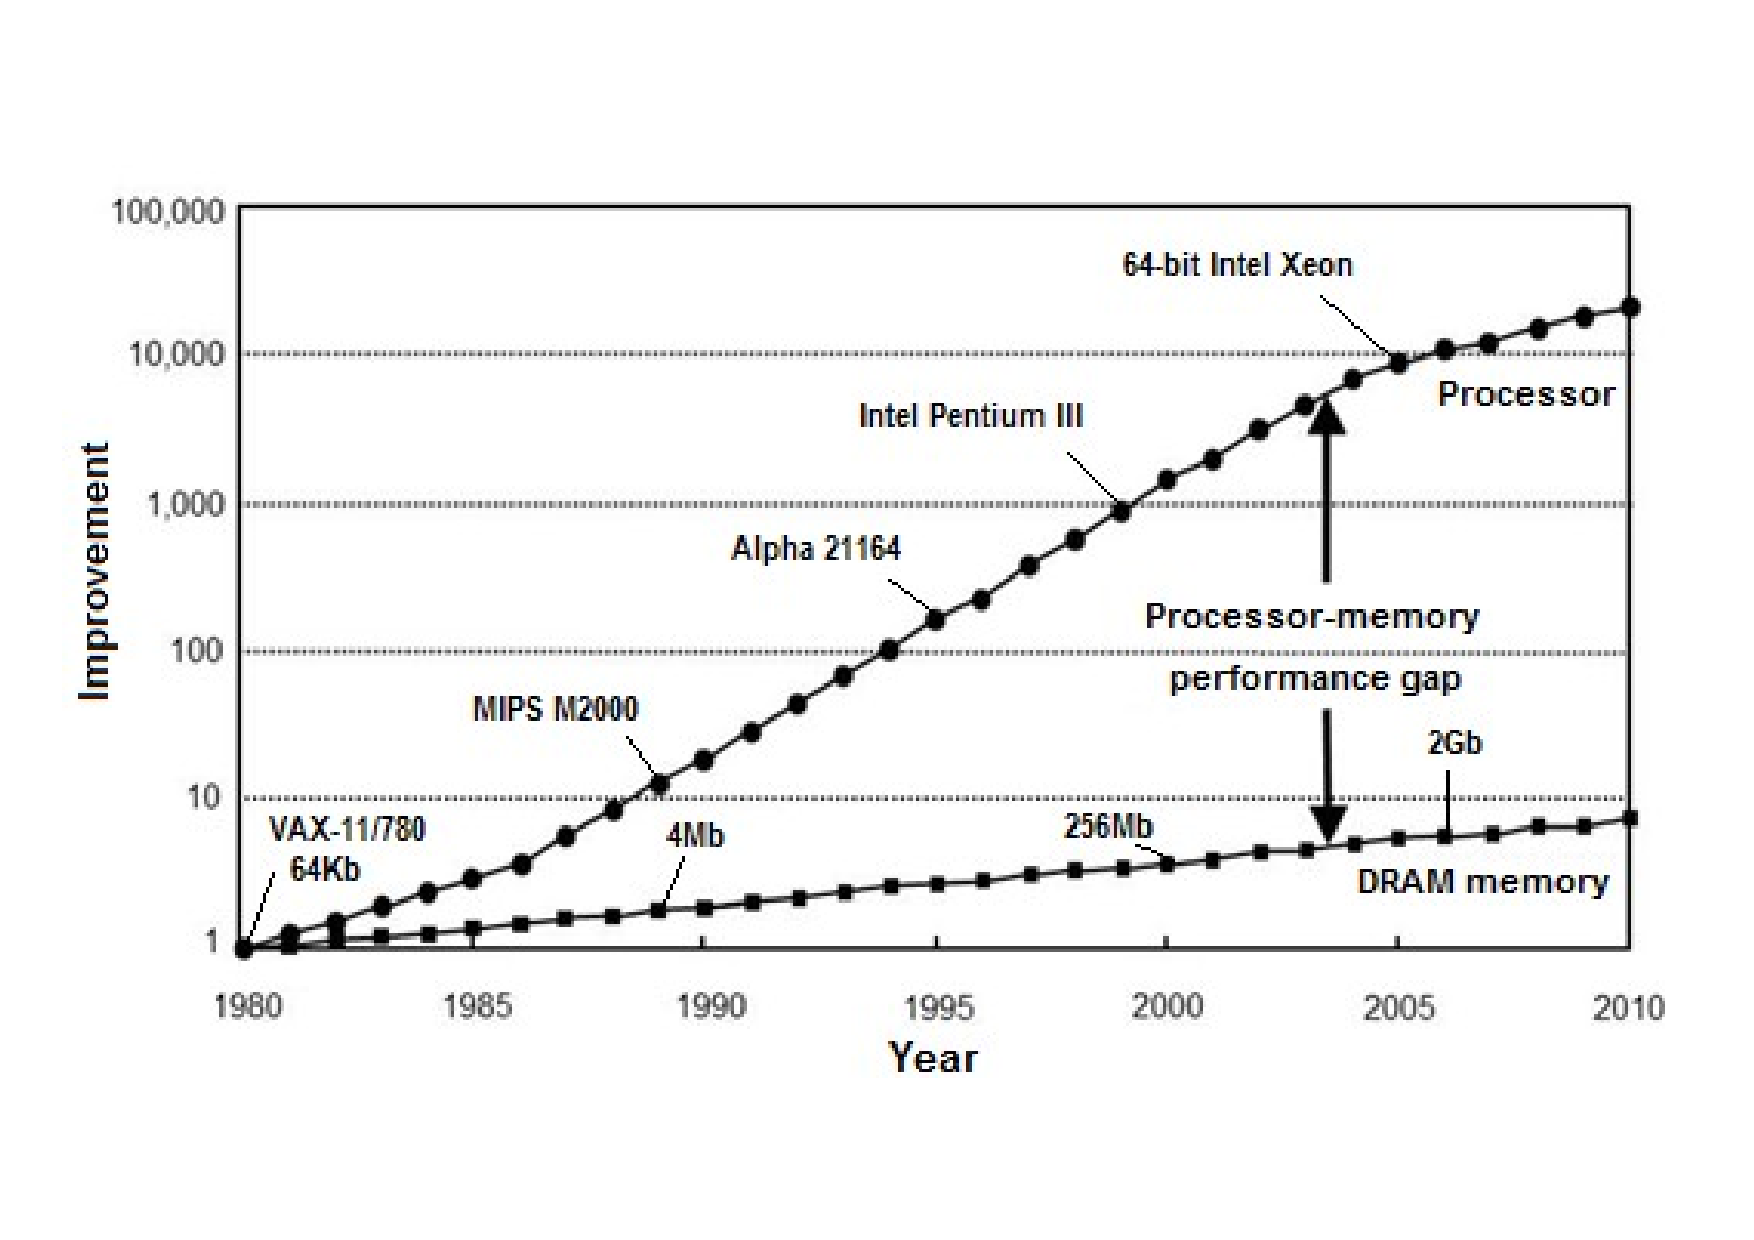
\includegraphics[scale=0.2]{processor_memory_gap.pdf}
    			\caption{Processor-Memory gap \cite{cpu-mem-gap}}
        		\label{fig:processor memory gap}
			\end{figure}
		\end{column}
	\end{columns}
\end{frame}

\begin{frame}
	\navframetitle{Memory Hierarchy}

	\begin{columns}
		\begin{column}{0.5\textwidth}
			\begin{itemize}
				\item To reduce processor-memory gap order memory in a hierarchy
				\item Trade off between cost, latency and bandwidth
				\item How to move data between the levels? 
			\end{itemize}
		\end{column}
		\begin{column}{0.5\textwidth}
			\begin{figure}[ht]
    			\centering
    			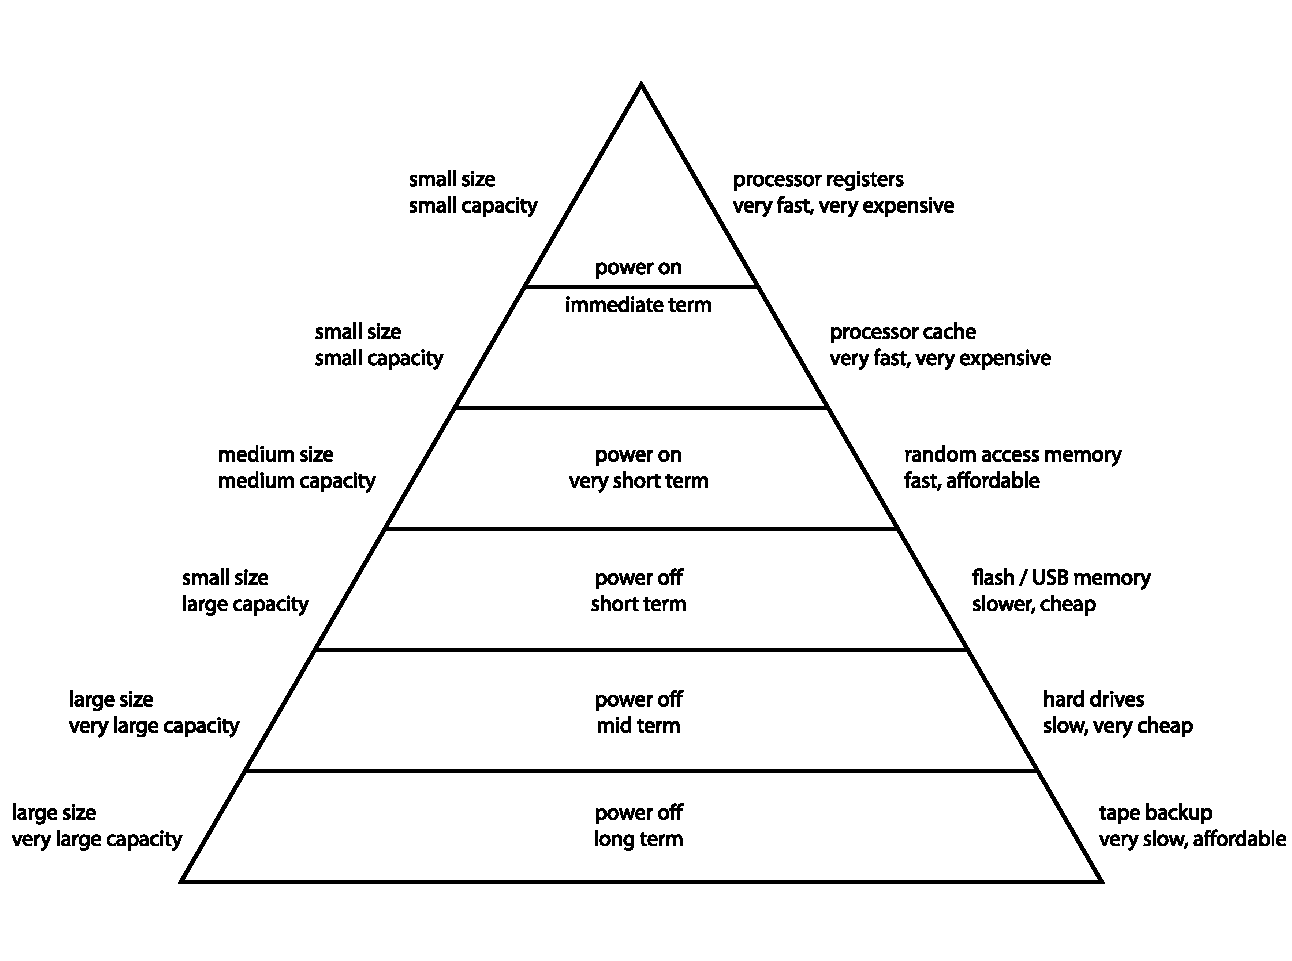
\includegraphics[scale=0.3]{ComputerMemoryHierarchy.pdf}
    			\caption{Memory Hierarchy \cite{wikiMemoryHierarchy}}
        		\label{fig:memory hierarchy}
			\end{figure}
		\end{column}
	\end{columns}
\end{frame}

\begin{frame}
	\navframetitle{Caching vs Tiered Storage}
	
	\begin{itemize}
		\item Similarities:
		\begin{itemize}
			\item Move data to faster storage 			
			\item Reduce latency and increase bandwidth
			\item Use of a policy  
		\end{itemize}		 
		\item But Tiered Storage actually move data
		\item Caching works with copies and can use cache lines
		\item Can be used together
	\end{itemize}
\end{frame}

\begin{frame}
	\navframetitle{Contribution}
	
	\begin{itemize}
		\item Implementation and Evaluation of different cache replacement policies for a copy on write optimized 
				hierarchical storage stack
		\item Affects of copy-on-write on cache performance
		\item Recommendation for certain use cases
	\end{itemize}
\end{frame}

\section{Background}
\label{sec:background}

\begin{frame}
	\navframetitle{$B^{\varepsilon}$-tree}

	\begin{columns}
		\begin{column}{0.5\textwidth}
			\begin{itemize}
				\item Write optimized variation of B-tree
				\item Uses buffer for each node, $B - B^{\varepsilon}$
				\item Comparable asymptotic cost but better for insertion operation
			\end{itemize}
		\end{column}
		\begin{column}{0.5\textwidth}
			\begin{figure}[ht]
    			\centering
    			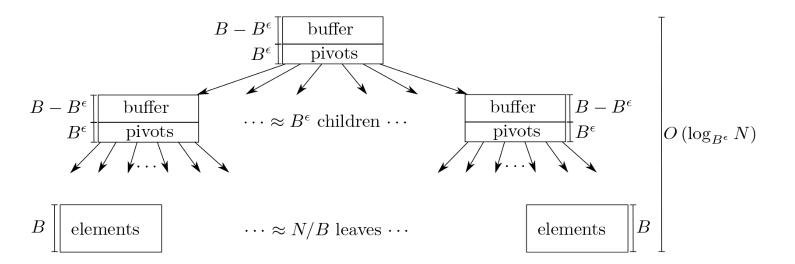
\includegraphics[scale=0.25]{B-epsilon_structure.png}
    			\caption{Structure $B^{\varepsilon}$-tree from \cite{bender2015introduction}}
        		\label{fig:structure B-epsilon-tree}
			\end{figure}			
		\end{column}
	\end{columns}
\end{frame}

\begin{frame}
	\navframetitle{Haura}
	
	\begin{columns}
		\begin{column}{0.5\textwidth}
			\begin{itemize}
				\item Hierarchical storage stack
				\item Key-value and object interface
				\item Designed for research
				\item Structured in layers
				\item Used directly or through wrapper
			\end{itemize}
		\end{column}
		\begin{column}{0.5\textwidth}
			\begin{figure}[ht]
    			\centering
    			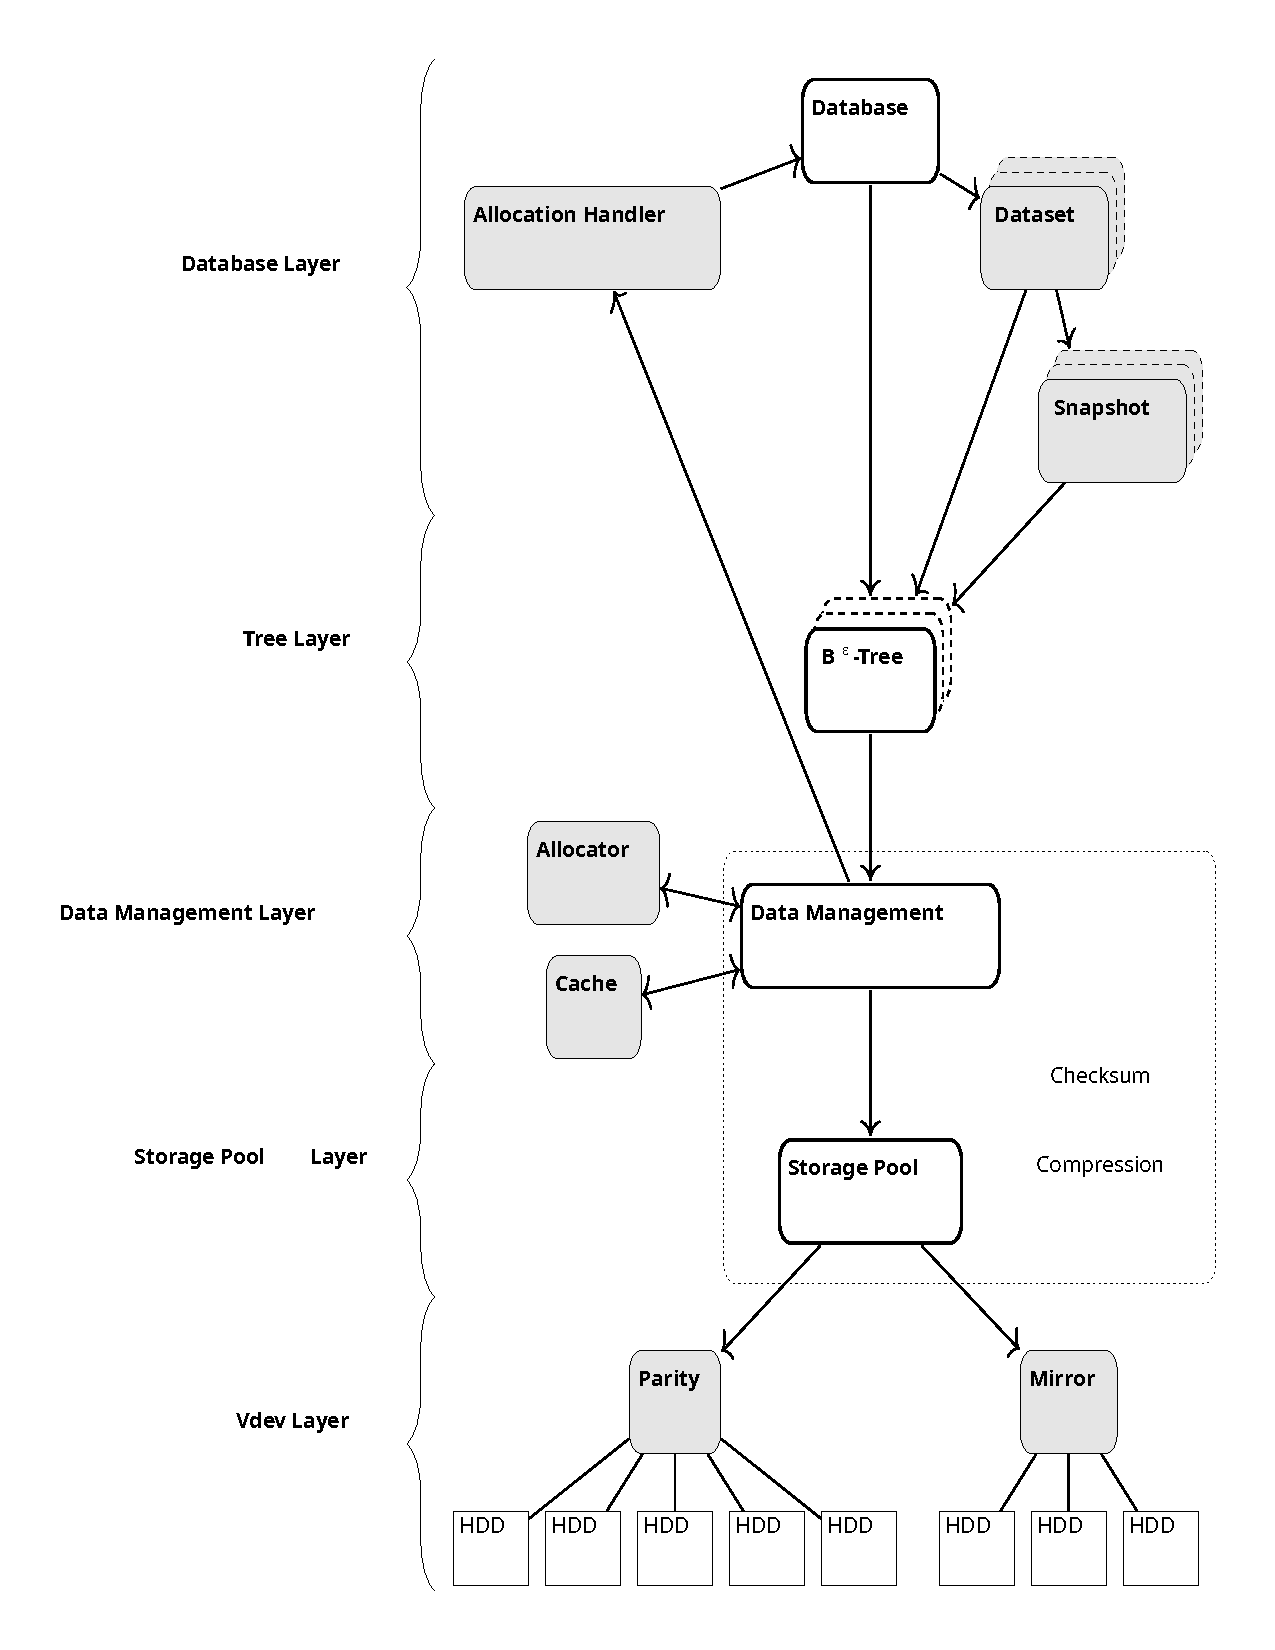
\includegraphics[scale=0.2]{overview_haura_level.pdf}
    			\caption{Structure Haura \cite{wiedemann2018modern}}
        		\label{fig:structure Haura}
			\end{figure}
		\end{column}
	\end{columns}
\end{frame}

\begin{frame}
	\navframetitle{Cache Replacement Policies}

	\begin{itemize}
		\item Used to manage Cache
		\item Decide which entries should be evicted
		\item Can use additional metadata or data structures, or both
		\item Early developed policies:
		\begin{itemize}
			\item Bélády’s algorithm
			\item FIFO
			\item LRU
			\item LFU
		\end{itemize}
	\end{itemize}
\end{frame}

\begin{frame}
	\navframetitle{Improved Cache Replacement Policies}

	\begin{itemize}
	\item Early developed policies have drawbacks:
	\begin{itemize}
		\item Bélády’s algorithm -> only theoretically useful
		\item FIFO -> Bélády’s anomaly
		\item LRU -> problems with weak locality, like loops and scans
		\item LFU -> high overhead and only for skewed access distributions
	\end{itemize}
	\item Several strategies to improve on these:
	\begin{itemize}
		\item Explicit user-level hints
    	\item Using deeper history information
    	\item Detection of access patterns
    	\item Using ml-techniques
	\end{itemize}
	\end{itemize}
\end{frame}

\section{Design and Implementation}
\label{sec:design}

\begin{frame}
	\navframetitle{Overview}

	\begin{columns}
		\begin{column}{0.5\textwidth}
			\begin{itemize}
				\item DMU and DML state cycle influences the implementation
				\item Pinned entries 
				\item Variable sized cache entries	
				\item Selected policies follow the strategies for improved policies
				\item All clock-based due to better scalability and low overhead
			\end{itemize}
		\end{column}
		\begin{column}{0.5\textwidth}
			\begin{figure}[ht]
    			\centering
    			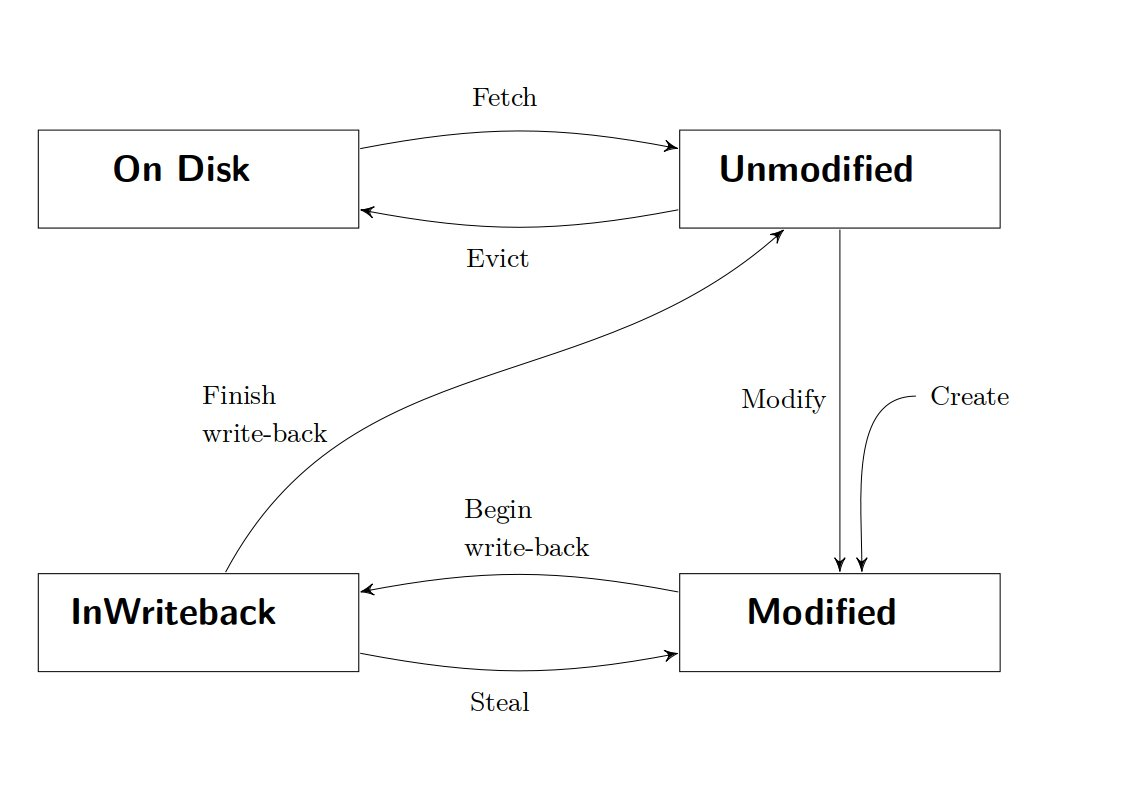
\includegraphics[scale=0.2]{DML_state_cycle.jpg}
    			\caption{DML state cycle, \cite{wiedemann2018modern}}
        		\label{fig:DML state cycle}
			\end{figure}			
		\end{column}
	\end{columns}
\end{frame}

\begin{frame}
	\navframetitle{CLOCK}

	\begin{columns}
		\begin{column}{0.5\textwidth}
			\begin{itemize}
				\item Introduced in \cite{corbato1968paging}				
				\item LRU approximation
				\item Was already implemented
				\item Uses a circular linked list and a "hand" pointer
				\item One reference bit per entry
				\item Pinned entries will be skipped
			\end{itemize}
		\end{column}
		\begin{column}{0.5\textwidth}
			\begin{figure}[ht]
    			\centering
    			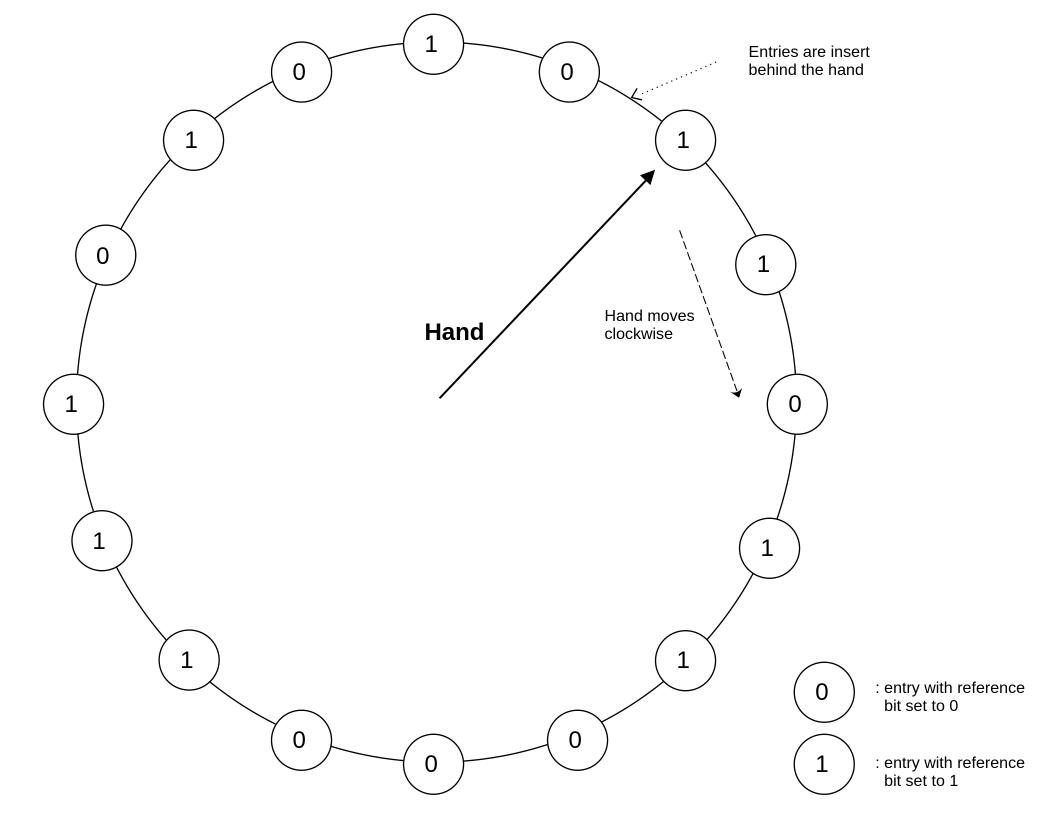
\includegraphics[scale=0.2]{clock.jpg}
    			\caption{Example for circular list in CLOCK.}
        		\label{fig:circular list for CLOCK}
			\end{figure}			
		\end{column}
	\end{columns}
\end{frame}

\begin{frame}
	\navframetitle{GCLOCK}
	
	\begin{itemize}
		\item Introduced in \cite{smith1978sequentiality}				
		\item Generalization of CLOCK 
		\item Uses more historical information
		\item Uses a circular linked list and a "hand" pointer
		\item Reference counter instead of reference bit, $k = 2$
		\item Pinned entries will be skipped
	\end{itemize}	
\end{frame}

\begin{frame}
	\navframetitle{CLOCK-PRO}

	\begin{columns}
		\begin{column}{0.5\textwidth}
			\begin{itemize}
				\item Introduced in \cite{jiang2005clock}			
				\item Combines LIRS with CLOCK
				\item Detect access patterns
				\item Categorize entries in hot and cold
				\item Uses non-resident (ghost) entries
				\item Modified eviction, pinned entries reinsert
				\item Non-resident cold entries not changed to hot entries due to DMU!
			\end{itemize}
		\end{column}
		\begin{column}{0.5\textwidth}
			\begin{figure}[ht]
    			\centering
    			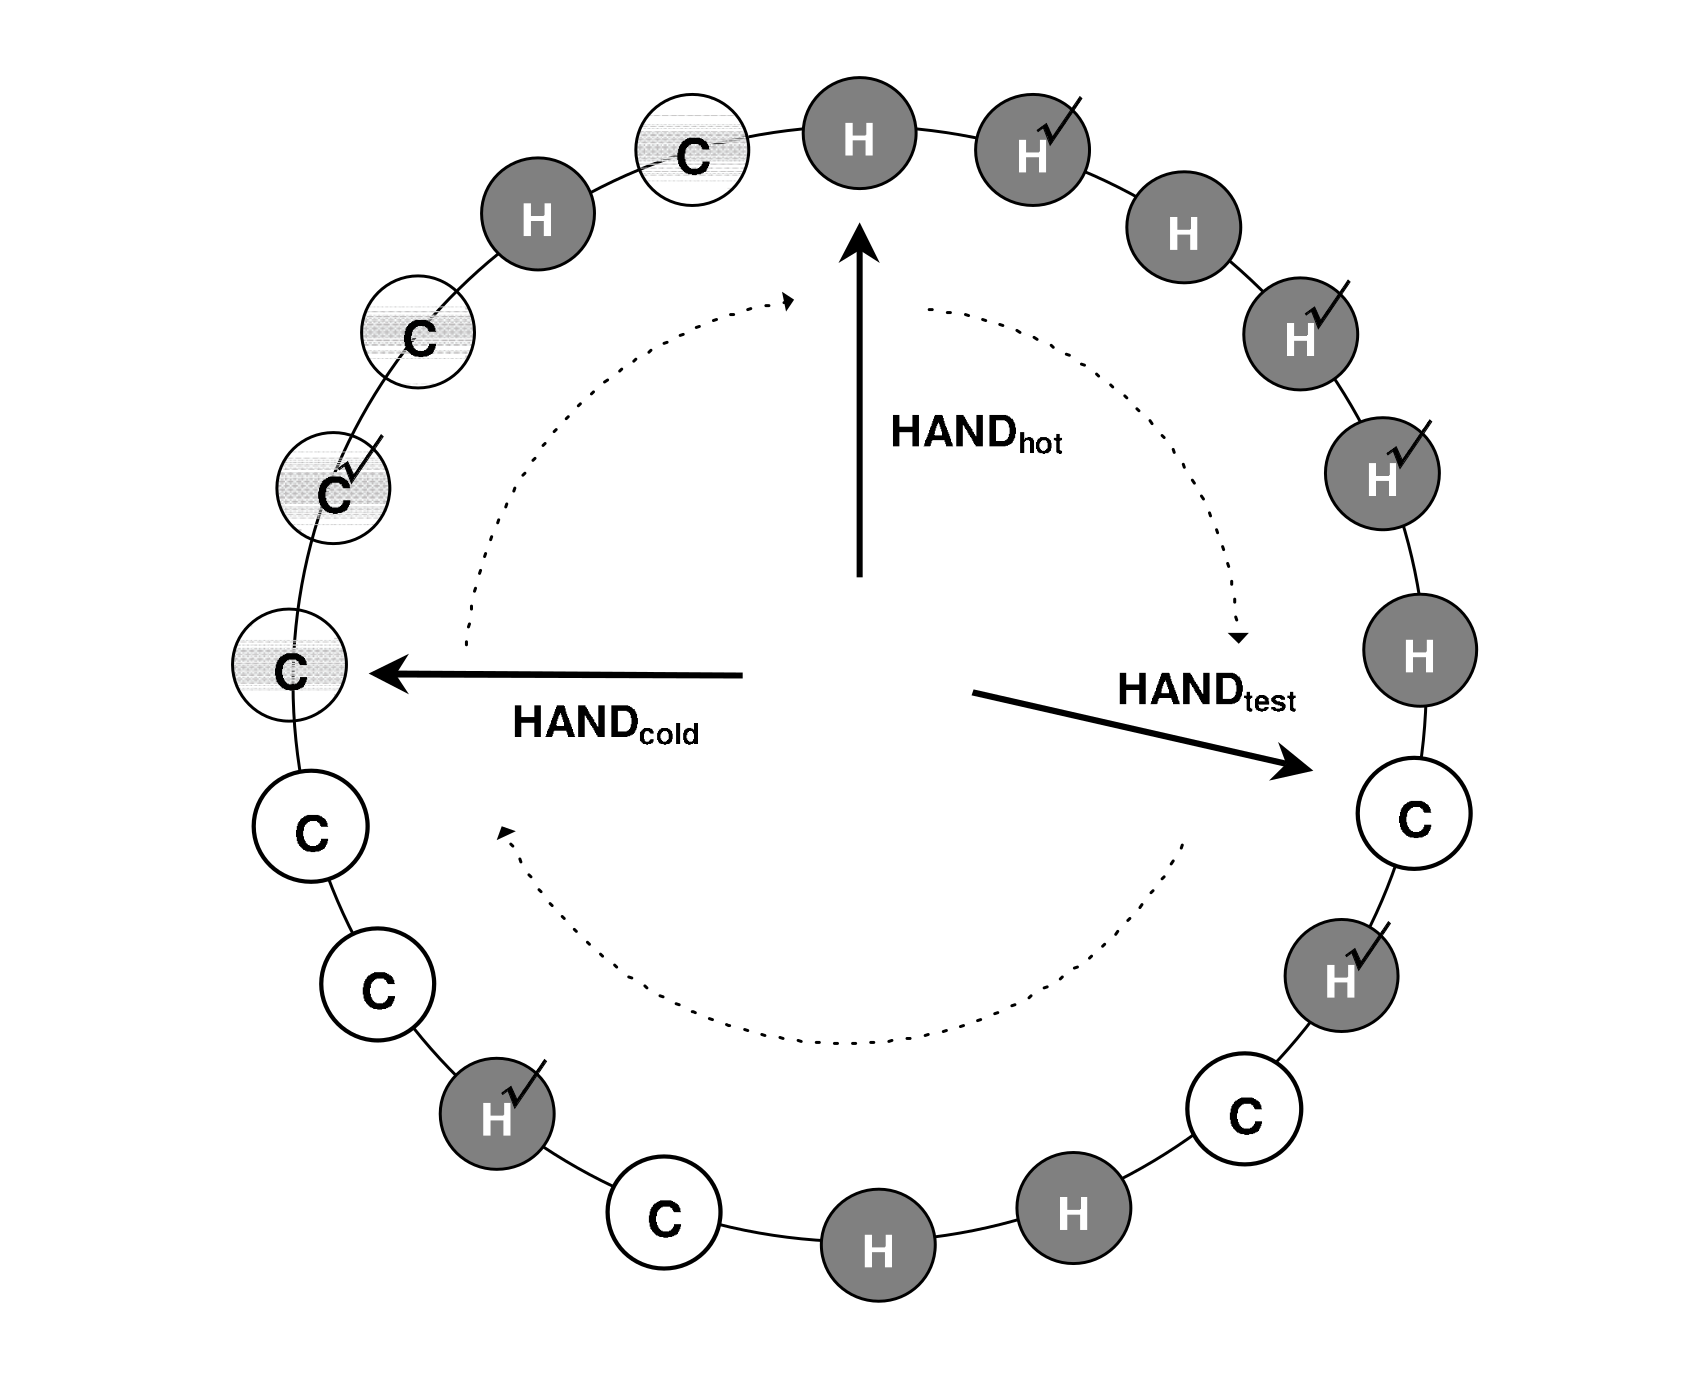
\includegraphics[scale=0.1]{clock_pro.png}
    			\caption{Example of the circular list for CLOCK-Pro. Hot entries marked with "H", cold entries with "C" and non-resident cold entries are shadowed.
    The "$\sqrt{}$" marks referenced entries.}
        		\label{fig:clock in clock-pro}
			\end{figure}			
		\end{column}
	\end{columns}
\end{frame}

\begin{frame}
	\navframetitle{ML-CLOCK}

\begin{itemize}
	\item Introduced in \cite{cho2021ml}	
	\item ML-learning technique
	\item Uses single-layer perceptron
	\item Uses frequency and recency information
	\item 2 clocks used clean and dirty
	\item Ghost queue for learning 
	\item Tries to minimize write operations
	\item Pinned entries skipped
	\item Modification no ghost entry reinsert to clock
\end{itemize}	
\end{frame}

\section{Evaluation}
\label{sec:evaluation}

\begin{frame}[fragile]
	\navframetitle{Methodology}

	\begin{itemize}
		\item Used Ovgu FIN Cluster with CephFS as secondary storage
		\item Used fio 3.33 to generate synthetic random I/O workloads
		\item Random distributions: zipf, normal, zoned and uniform
		\item Read-only and mixed Read-write, with 90\% read and 50\% reads, workloads
		\item Single and multi threaded, up to 16 threads
		\item Cache size is small with 1GB
 	\end{itemize}
\end{frame}

\begin{frame}[fragile]
	\navframetitle{Single Threaded Benchmarks}
	
	\begin{columns}
		\begin{column}{0.5\textwidth}
			\begin{itemize}
				\item Read-only benchmarks CLOCK and GCLOCK highest performance
				\item Read-only CLOCK-Pro shows worst performance
				\item Mixed benchmarks ML-Clock best performance
				\item CLOCK, GCLOCK and CLOCK-Pro nearly equal performance
				\item Increased write operations leads to lower hit rate
			\end{itemize}
		\end{column}
		\begin{column}{0.5\textwidth}
			\begin{figure}[ht]
    			\centering
    			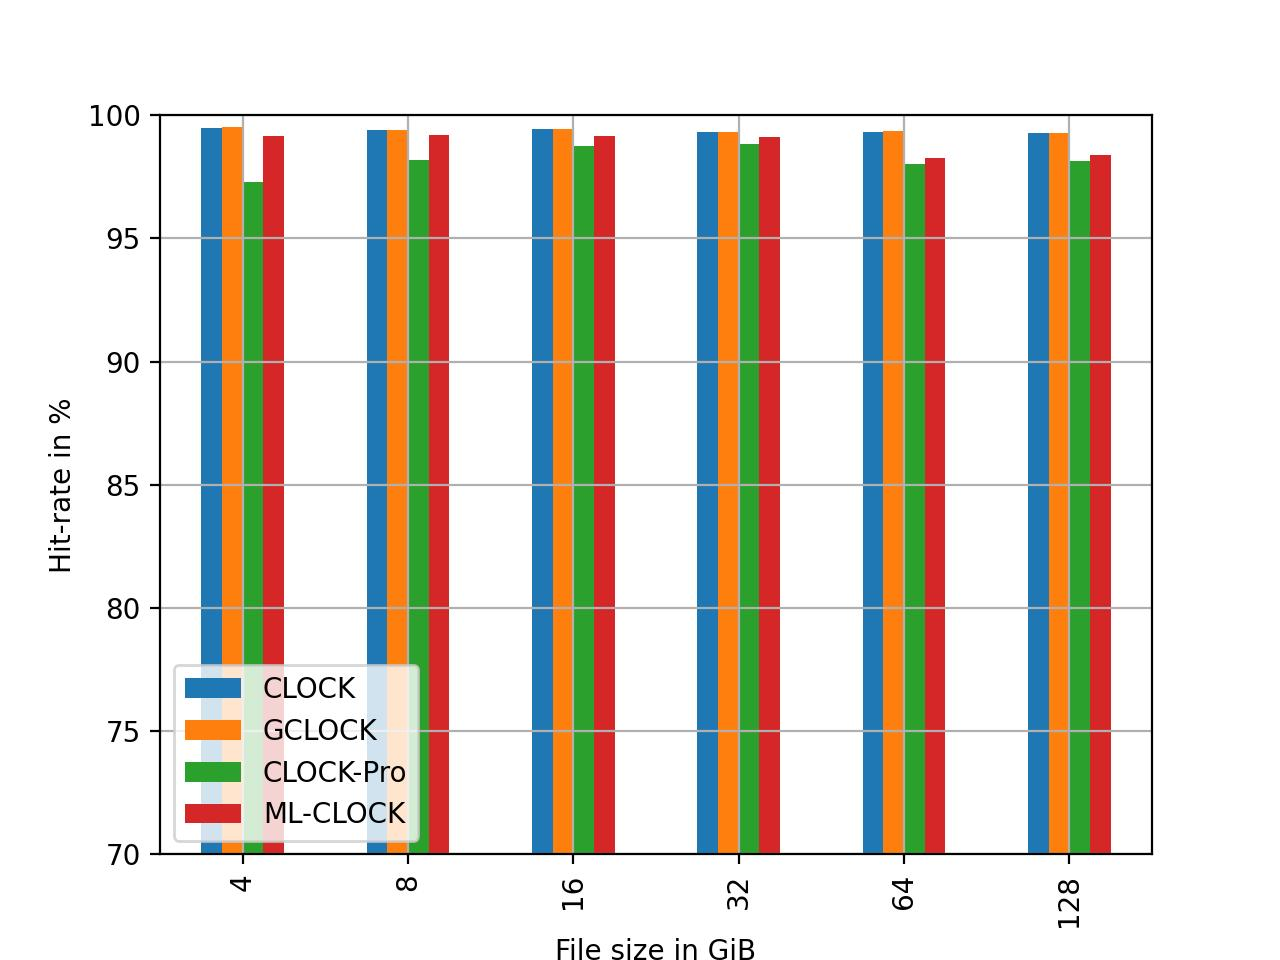
\includegraphics[width=\textwidth]{randread_zipf.jpg}
        		\caption{Read-only, zipf-distribution}
        		\label{fig:single randread zipf}
			\end{figure}			
		\end{column}
	\end{columns}
\end{frame}

\begin{frame}[fragile]
	\navframetitle{Single Threaded Benchmarks}

	\begin{columns}
		\begin{column}{0.5\textwidth}
			\begin{figure}
				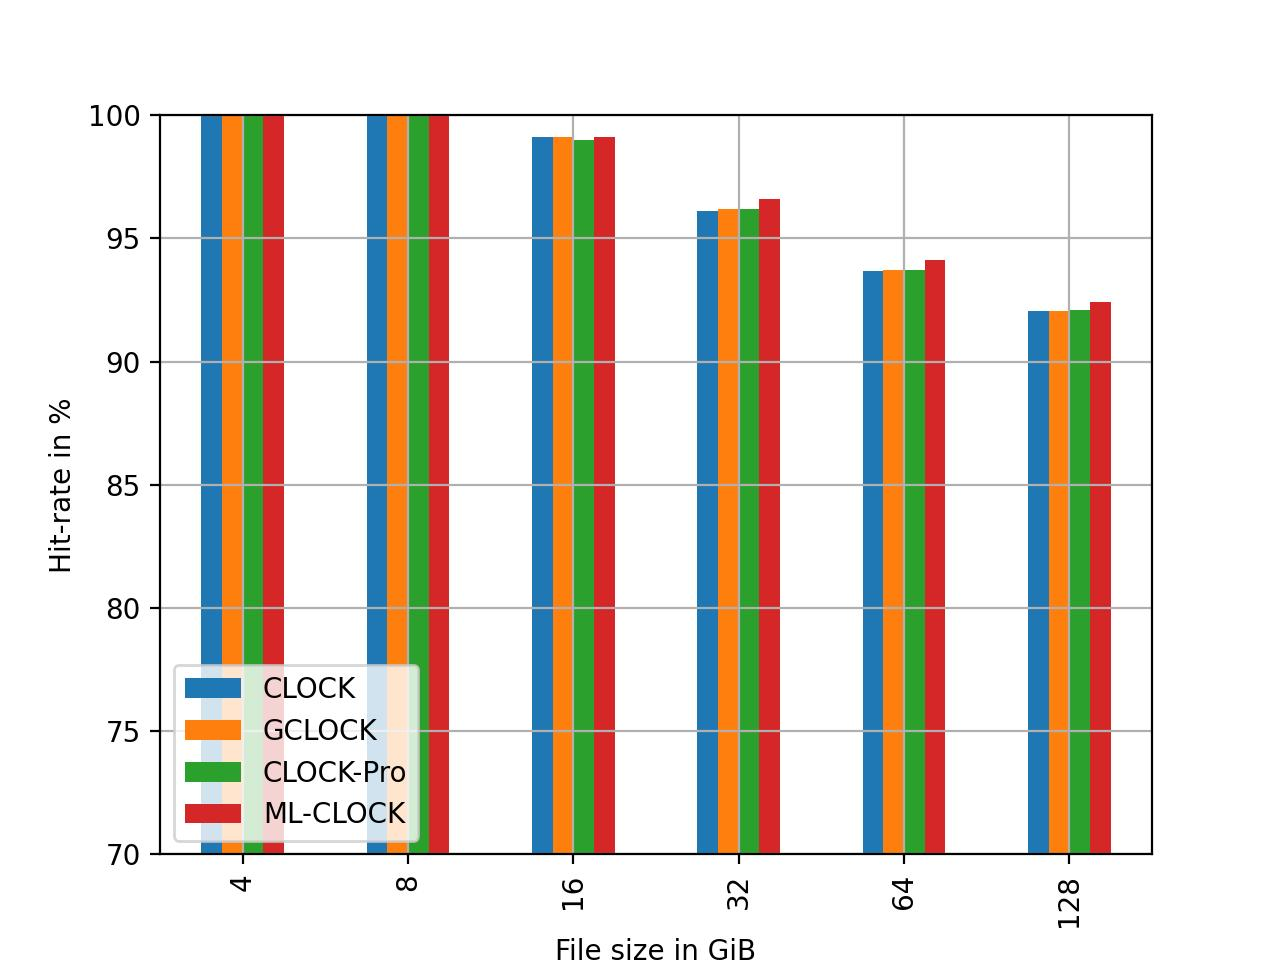
\includegraphics[width=\textwidth]{rw_90to10_zoned.jpg}
        		\caption{Mixed, 90\% reads, zoned-distribution}
        		\label{fig:single rw_90to10  zoned}
			\end{figure}
		\end{column}
		\begin{column}{0.5\textwidth}
			\begin{figure}[ht]
    			\centering
    			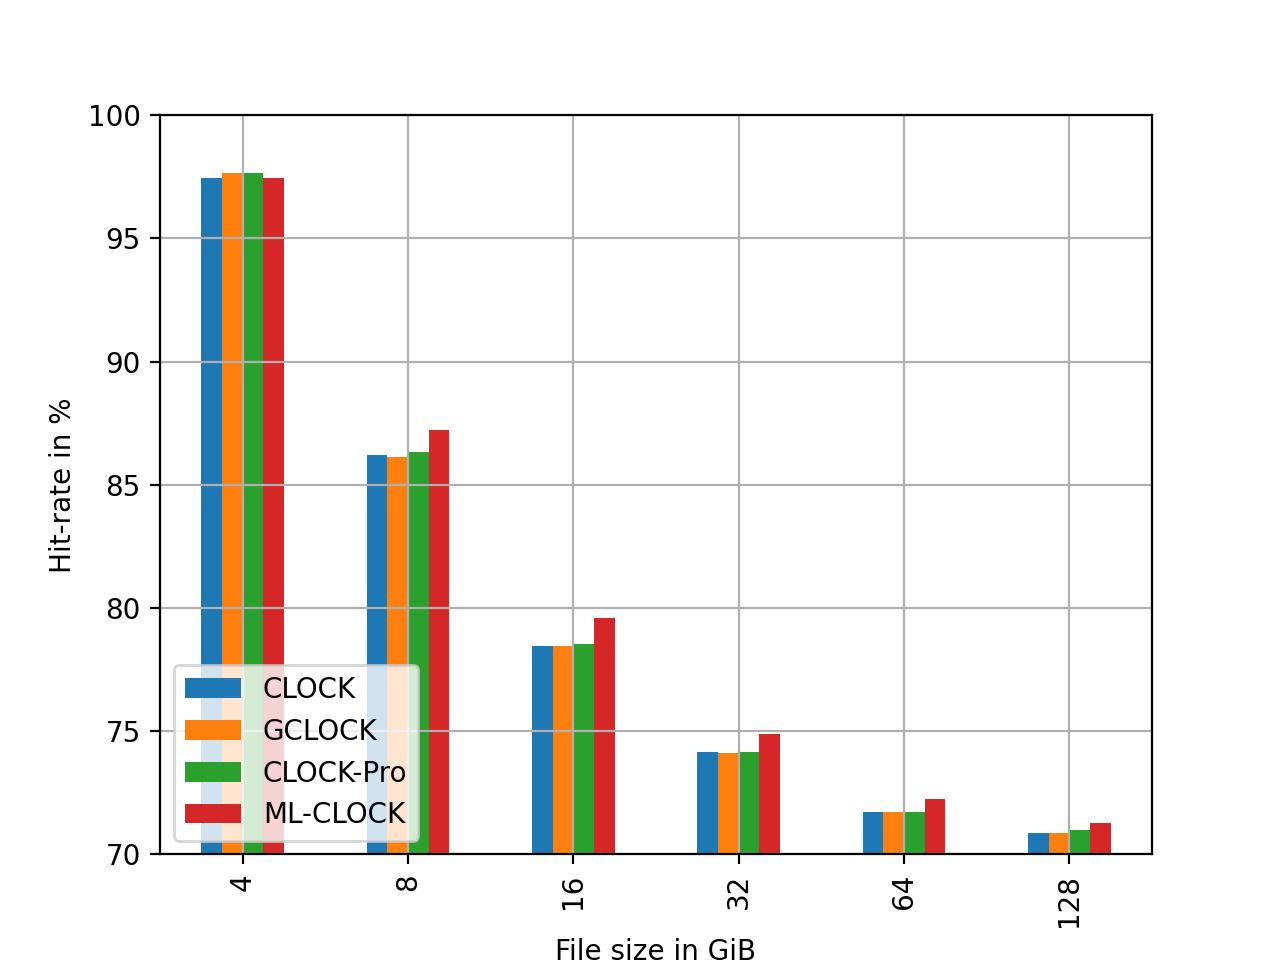
\includegraphics[width=\textwidth]{rw_50to50_normal.jpg}
        		\caption{Mixed, 50\% reads, normal-distribution}
        		\label{fig:single rw_90to10  normal}
			\end{figure}			
		\end{column}
	\end{columns}
\end{frame}

\begin{frame}[fragile]
	\navframetitle{Multi Threaded Benchmarks}

	\begin{columns}
		\begin{column}{0.5\textwidth}
			\begin{itemize}
				\item Result not as clear as single threaded benchmarks
				\item Read-only benchmarks CLOCK and GCLOCK highest performance
				\item Read-only CLOCK-Pro worst performance
				\item Mixed no clear best policy
				\item Mixed ML-CLOCK good performance for lower thread count
				\item Mixed CLOCK-Pro better performance for higher thread count
			\end{itemize}
		\end{column}
		\begin{column}{0.5\textwidth}
			\begin{figure}[ht]
    			\centering
    			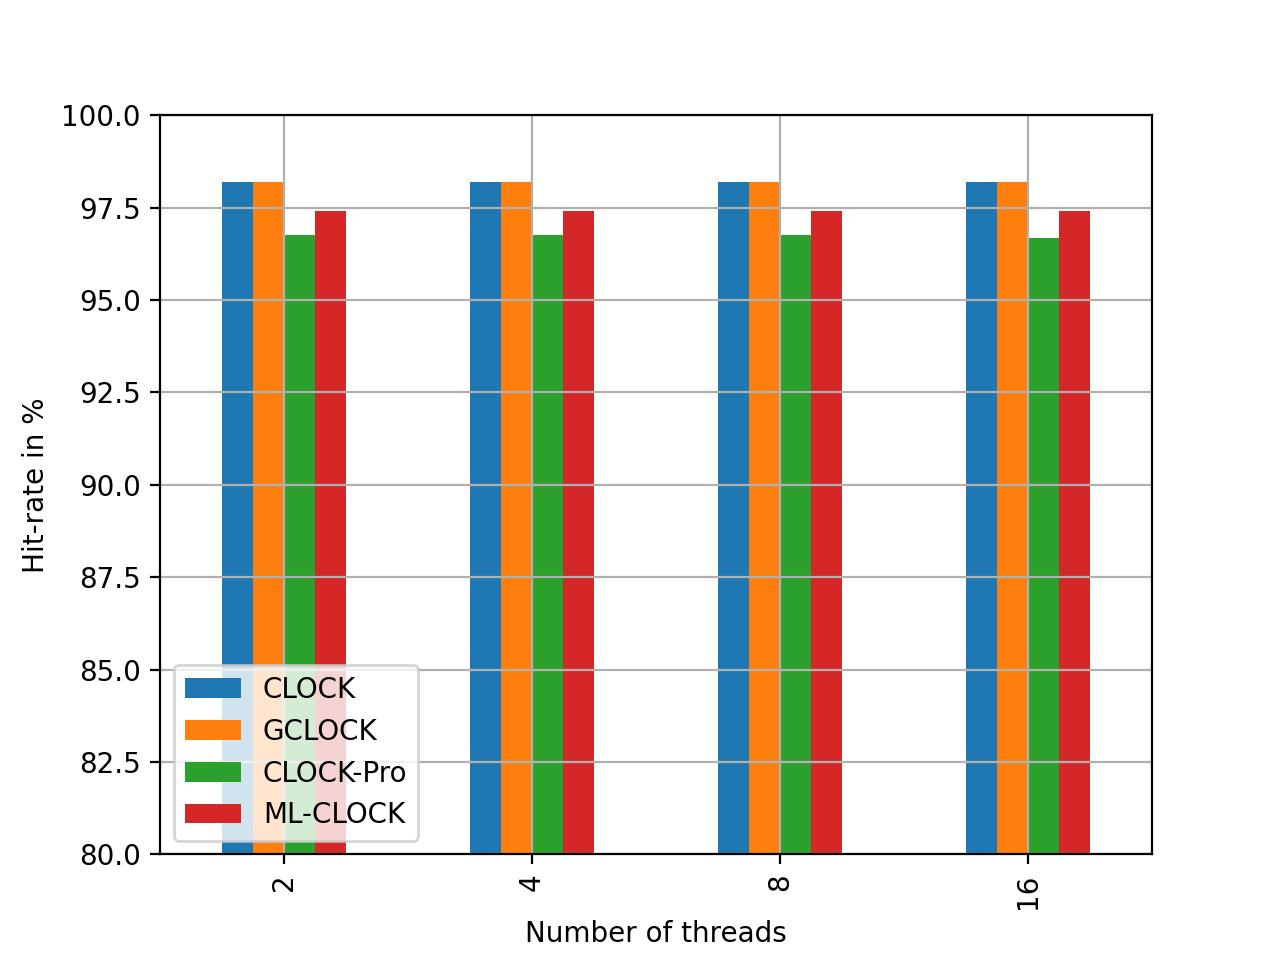
\includegraphics[width=\textwidth]{multi_128_gb_randread_normal.jpg}
        		\caption{Read-only, normal-distribution, 128 GiB file size}
        		\label{fig:rw_90to10 128 normal}
			\end{figure}			
		\end{column}
	\end{columns}
\end{frame}

\begin{frame}[fragile]
	\navframetitle{Multi Threaded Benchmarks}

	\begin{columns}
		\begin{column}{0.5\textwidth}
			\begin{figure}[ht]
    			\centering
    			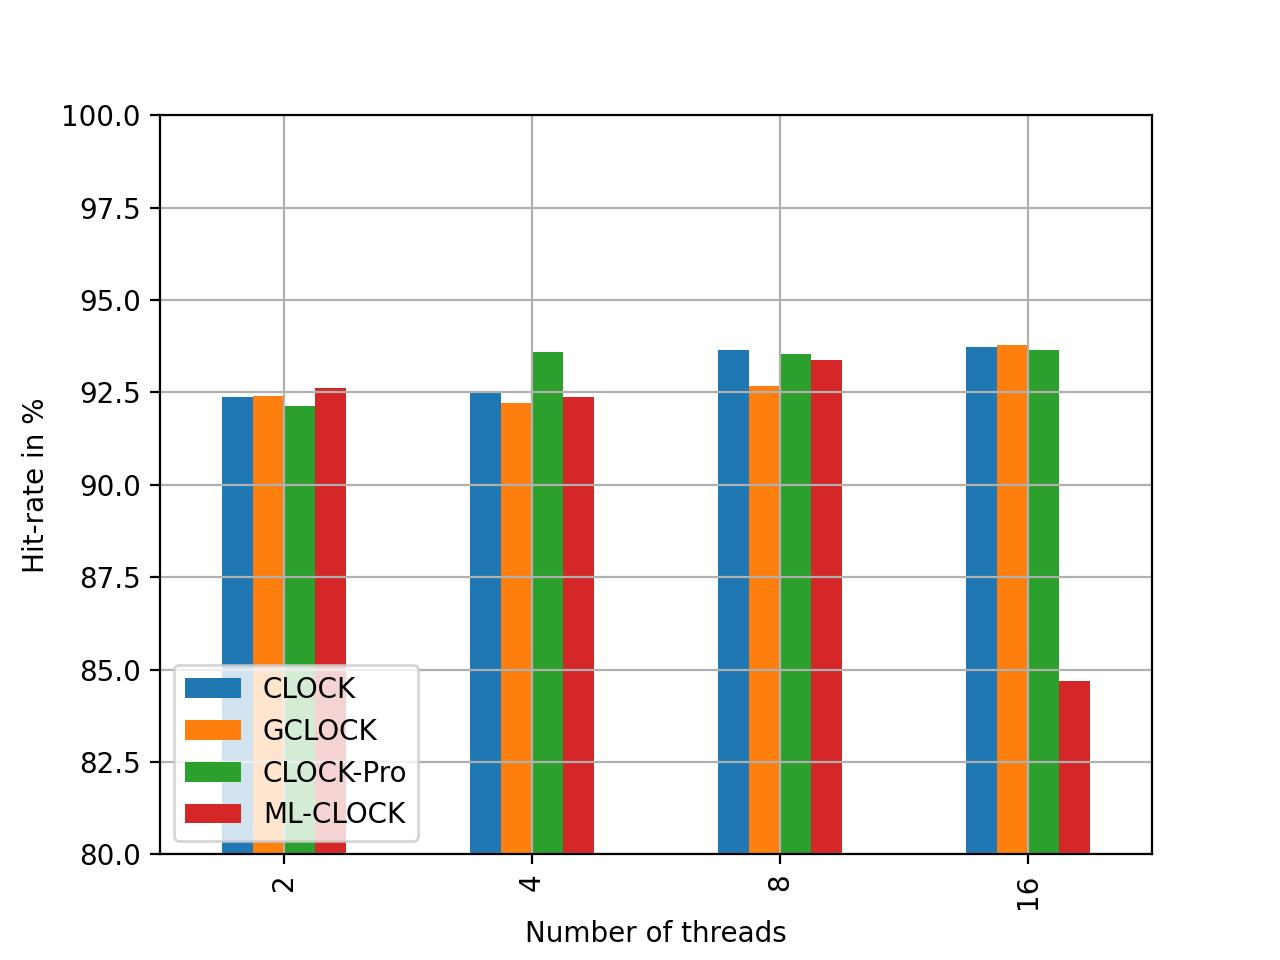
\includegraphics[width=\textwidth]{multi_128_gb_rw_90to10_zoned.jpg}
        		\caption{Mixed, 90\% reads, zoned-distribution, 128 GiB file size}
        		\label{fig:rw_90to10 128 zoned}
			\end{figure}
		\end{column}
		\begin{column}{0.5\textwidth}
			\begin{figure}[ht]
    			\centering
    			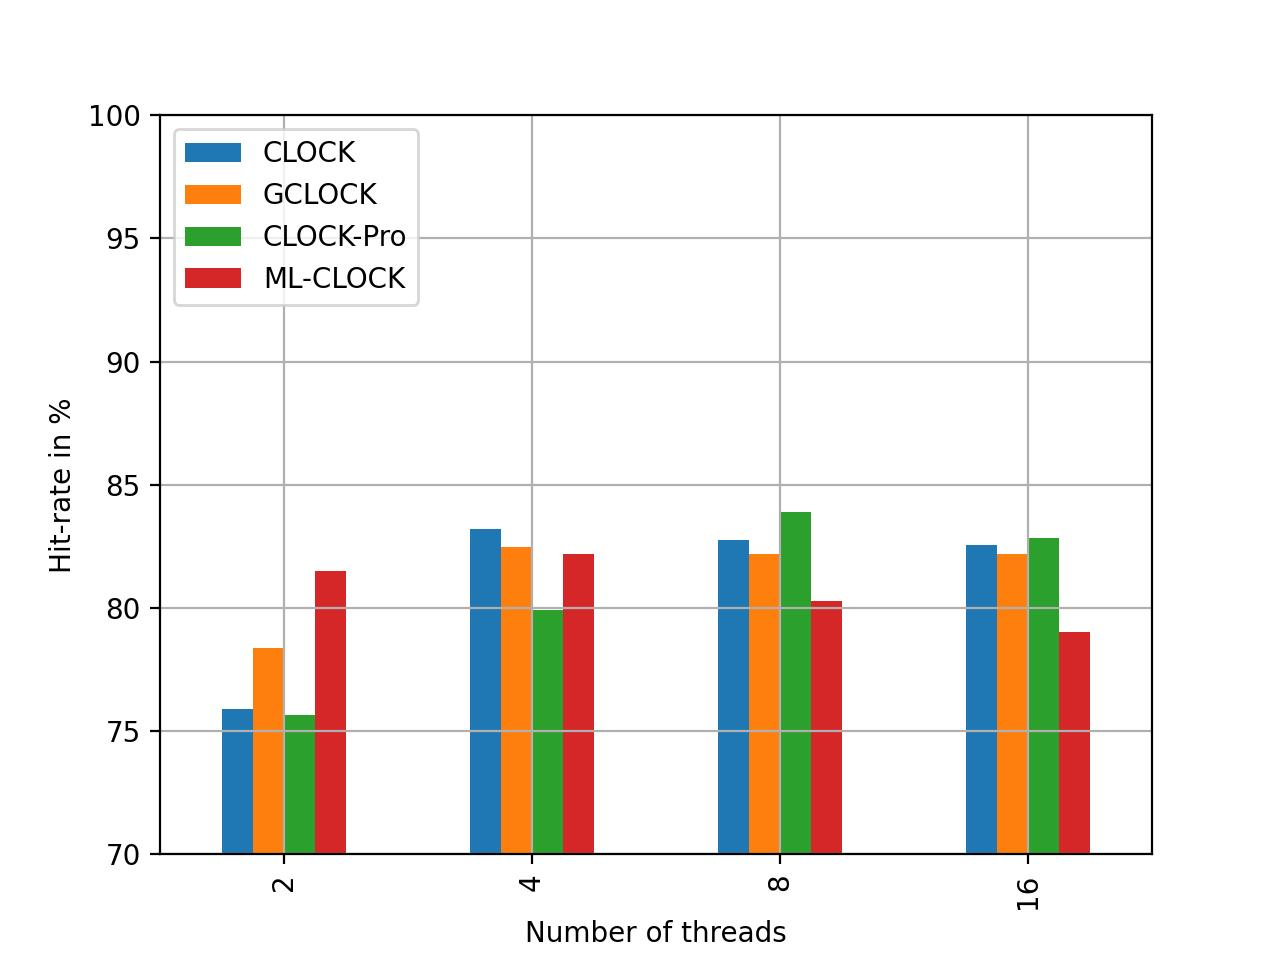
\includegraphics[width=\textwidth]{multi_64_gb_rw_50to50_normal.jpg}
        		\caption{Mixed, 50\% reads,normal-distribution, 64 GiB file size}
        		\label{fig:rw_50to50 64 normal}
			\end{figure}			
		\end{column}
	\end{columns}
\end{frame}

\begin{frame}[fragile]
	\navframetitle{Multi Threaded Benchmarks}

	\begin{columns}
		\begin{column}{0.5\textwidth}
			\begin{figure}[ht]
    			\centering
    			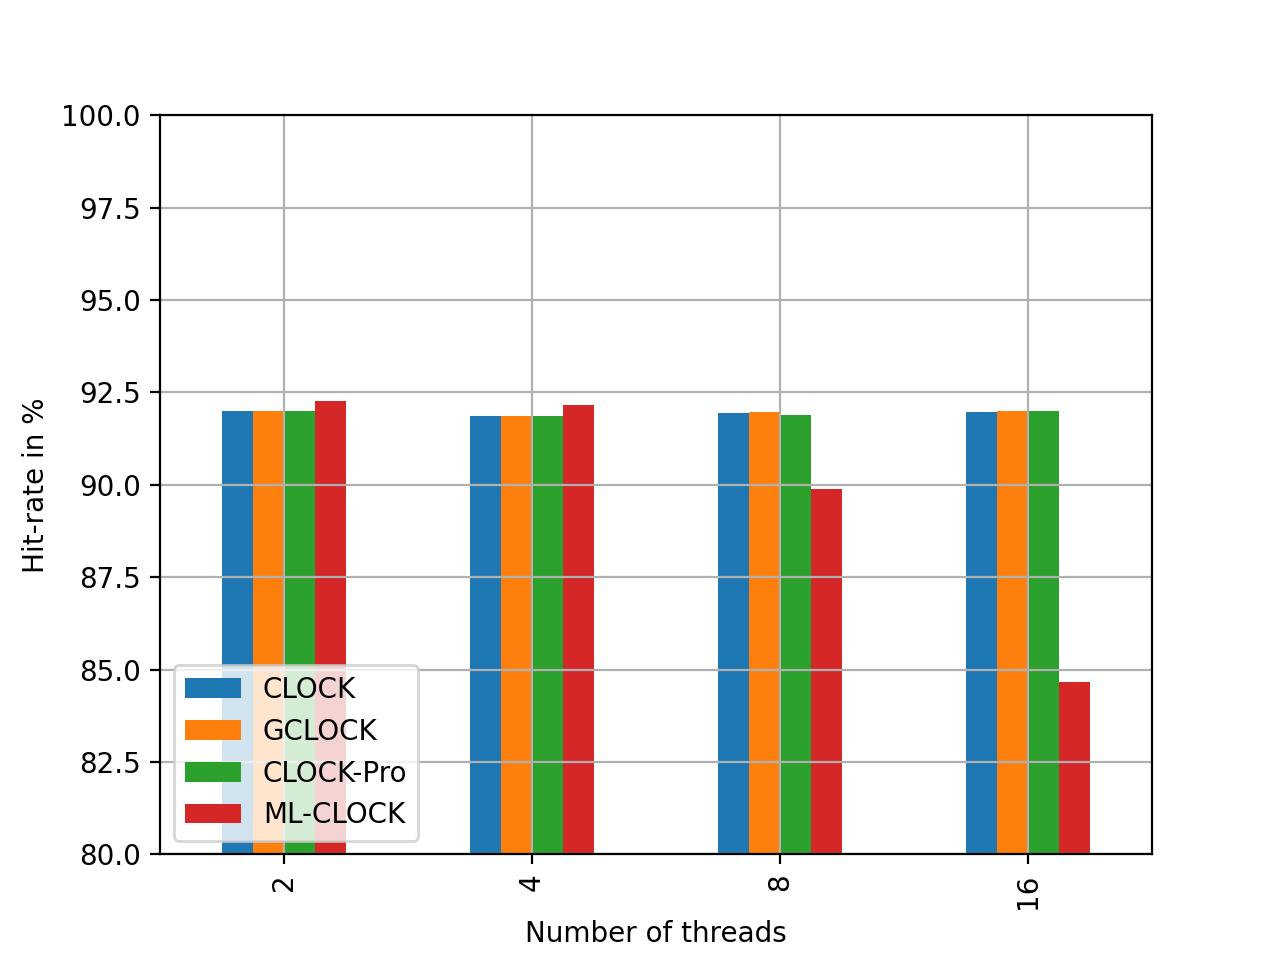
\includegraphics[width=\textwidth]{multi_128_gb_rw_90to10_uniform.jpg}
        		\caption{Mixed, 90\% reads, uniform-distribution, 128 GiB file size}
        		\label{fig:rw_90to10 128 uniform}
			\end{figure}
		\end{column}
		\begin{column}{0.5\textwidth}
			\begin{figure}[ht]
    			\centering
    			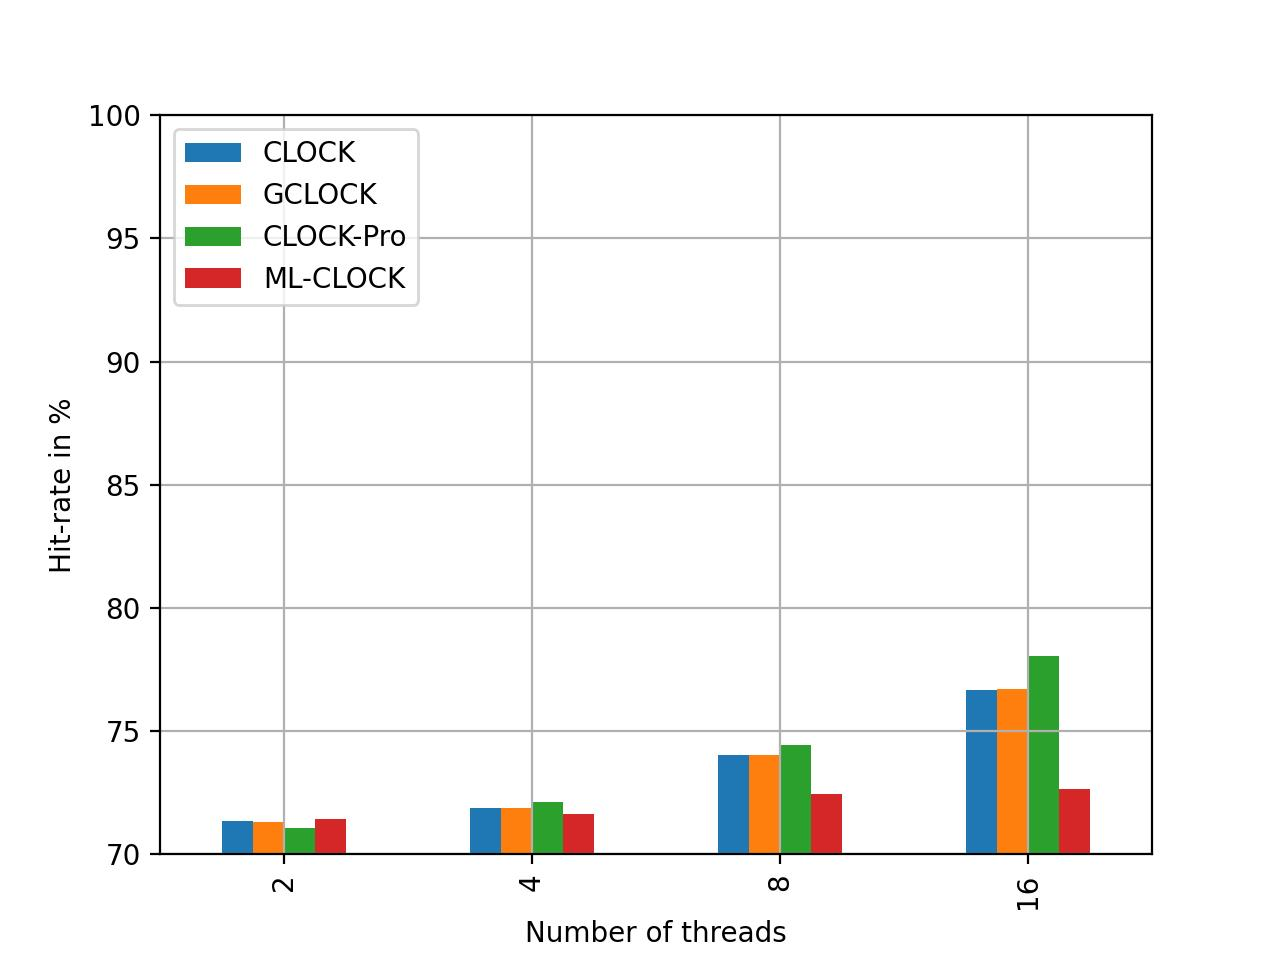
\includegraphics[width=\textwidth]{multi_128_gb_rw_50to50_uniform.jpg}
        		\caption{Mixed, 50\% reads, uniform-distribution, 128 GiB file size}
        		\label{fig:rw_50to50 128 uniform}
			\end{figure}			
		\end{column}
	\end{columns}
\end{frame}

\section{Conclusion}
\label{sec:conclusion}

\begin{frame}
	\navframetitle{Conclusion}

	\begin{itemize}
		\item Increasing ratio of write operation reduces cache hit rate
		\item Single threaded workloads ML-CLOCK performs best, CLOCK and GCLOCK in read-only workload
		\item Multi threaded workloads no clear results
		\item ML-CLOCK shows good performance for low thread count
		\item CLOCK-Pro shows good performance for higher thread count
	\end{itemize}
\end{frame}

\begin{frame}
	\navframetitle{Future Work}
	
	\begin{itemize}
		\item Modify DMU and policies so that CLOCK-Pro and ML-CLOCK can work correctly
		\item Include application traces for evaluation
		\item Test if ML-CLOCK reduces write operation
		\item Test more cache replacement policies
		\item Extent test cases for multi threaded workloads
	\end{itemize}
\end{frame}

\appendix

\AtBeginSection[]{}
\AtBeginSubsection[]{}

\section{References}

\begin{frame}[allowframebreaks]
	\frametitle{References}

	\bibliographystyle{apalike}
	\bibliography{presentation}
\end{frame}

\end{document}